% fancytikzposter.tex, version 2.1
% Original template created by Elena Botoeva [botoeva@inf.unibz.it], June 2012
% 
% This file is distributed under the Creative Commons Attribution-NonCommercial 2.0
% Generic (CC BY-NC 2.0) license
% http://creativecommons.org/licenses/by-nc/2.0/ 


\documentclass{a0poster}

\usepackage{fancytikzposter} 


%%%%% --------- Change here if you want ---------- %%%%%
%% margin for the geometry package, must be changed before using the geometry package
%% default value is 4cm
\setmargin{2}

%% the space between the blocks
%% default value is 2cm
% \setblockspacing{2}

%% the height of the title stripe in block nodes, decrease it to save space
%% default value is 3cm
% \setblocktitleheight{3}

%% the number of columns in the poster, possible values 2,3
%% default value is 2
% \setcolumnnumber{3}

%% the space between two or more groups of authors from different institutions
%% used in \maketitle
% \setinstituteshift{10}

%% which template to use
%% N1 simple, standard look, with a colored background and gray boxes
%% N2 board with nodes
%% N3 another standard look
%% N4 envelope-like look
%% N5 with a wave-like head, original idea taken from
%%%% http://fc09.deviantart.net/fs71/f/2010/322/1/1/scientific_poster_by_nabuy-d333ria.jpg
%\usetemplate{5}

%% components of the templates
%% (the maximal possible numbers are mentioned as the parameters)
% \usecolortemplate{4}
% \usebackgroundtemplate{5}
% \usetitletemplate{2}
% \useblocknodetemplate{5}
% \useplainblocktemplate{4}
% \useinnerblocktemplate{2}


%% the height of the head drawing on top 
%% applicable to templates N3, 4 and 5
% \setheaddrawingheight{14}


%% change the basic colors
%\definecolor{myblue}{HTML}{008888} 
%\setfirstcolor{myblue}% default 116699
%\setsecondcolor{gray!80!}% default CCCCCC
%\setthirdcolor{red!80!black}% default 991111

%% change the more specific colors
% \setbackgrounddarkcolor{colorone!70!black}
% \setbackgroundlightcolor{colorone!70!}
% \settitletextcolor{textcolor}
% \settitlefillcolor{white}
% \settitledrawcolor{colortwo}
% \setblocktextcolor{textcolor}
% \setblockfillcolor{white}
% \setblocktitletextcolor{colorone}
% \setblocktitlefillcolor{colortwo} %the color of the border
% \setplainblocktextcolor{textcolor}
% \setplainblockfillcolor{colorthree!40!}
% \setplainblocktitletextcolor{textcolor}
% \setplainblocktitlefillcolor{colorthree!60!}
% \setinnerblocktextcolor{textcolor}
% \setinnerblockfillcolor{white}
% \setinnerblocktitletextcolor{white}
% \setinnerblocktitlefillcolor{colorthree}




%%% size of the document and the margins
%% A0
% \usepackage[margin=\margin cm, paperwidth=118.9cm, paperheight=84.1cm]{geometry} 
\usepackage[margin=\margin cm, paperwidth=84.1cm, paperheight=118.9cm]{geometry}
%% B1
% \usepackage[margin=\margin cm, paperwidth=70cm, paperheight=100cm]{geometry}



%% changing the fonts
%\usepackage{cmbright}
%\usepackage[default]{cantarell}
\usepackage{avant}
%\usepackage[math]{iwona}
\usepackage[math]{kurier}
\usepackage[utf8]{inputenc}
\usepackage[T1]{fontenc}


%% add your packages here
\usepackage{hyperref}
\usepackage{wrapfig}

%% custom configuration
\graphicspath{{img/}} % Specifies the directory where pictures are stored


\title{{\fontsize{72pt}{72pt}\selectfont Mise en \oe{}uvre d'une plateforme d'intégration continue pour un logiciel spatial}\\
  {\fontsize{52pt}{52pt}\selectfont TN09}
}
\author{{\fontsize{30pt}{30pt}\selectfont Centre CEA de Paris-Saclay — Institut de recherche sur les lois fondamentales de l'univers}\\
Guillaume \textsc{Jorandon}
}


\begin{document}

%%%%% ---------- the background picture ---------- %%%%%
%% to change it modify the macro \BackgroundPicture
\ClearShipoutPicture
\AddToShipoutPicture{\BackgroundPicture}

\noindent % to have the picture right in the center
\begin{tikzpicture}
  \initializesizeandshifts
  % \setxshift{15}
  % \setyshift{2}


  %% the title block, #1 - shift, the default value is (0,0), #2 - width, #3 - scale
  %% the alias of the title block is `title', so we can refer to its boundaries later
  \ifthenelse{\equal{\template}{1}}{ 
    \titleblock{47}{1}
  }{
    \titleblock{47}{1.5}
  }

  %% a logo can be added to the title block
  %% #1 - anchor relative to the title block, #2 - shift, #3 - width, #3 - file name
  % \ifthenelse{\equal{\template}{2}}{ 
  %   \addlogo[south west]{(2,0)}{6cm}{unibz_b.png}
  % }{
  %   \addlogo[south west]{(2,0)}{6cm}{unibz_w.png}
  % }

  \addlogo[north west]{(-14,-\blocktitleheight-2)}{12cm}{logo_utc}
  \addlogo[north east]{(12,-\blocktitleheight-1)}{10cm}{logo_cea}

  %% a block node, with the specified position (optional), title and the content
  %% #1 - where (optional), #2 - title, #3 - text
  %%%%%%%%%% ------------------------------------------ %%%%%%%%%%
  \blocknode%
  		{Contexte du stage}
		{\begin{tikzfigure}
\includegraphics[height=6cm]{logo_cea}\end{tikzfigure}
		\begin{itemize}
				\item Le CEA, un organisme \textbf{public} de recherche \textbf{scientifique}. Il travaille notamment autour de l'énergie nucléaire, des sciences fondamentales et de la recherche industrielle.
		\begin{tikzfigure}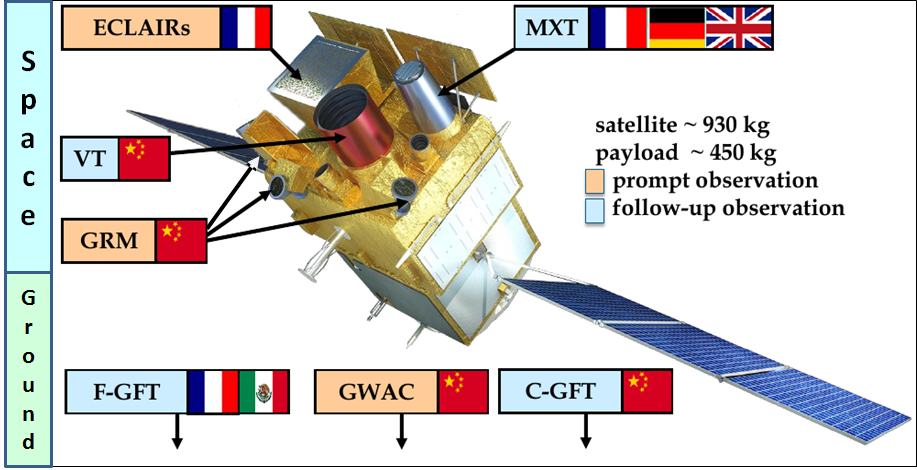
\includegraphics[height=16cm]{svom}\end{tikzfigure}
		\item SVOM, un projet franco-chinois de satellite de détection et d'étude des \textbf{sursauts gamma}.
		\end{itemize}}
  
  \calloutblock{($(box.south east)-(22,-1.5)$)}
  {($(box.south east)-(16,2)$)}
  {30cm}
  {
		  Émission brève et intense de rayons gamma en provenance de l'espace. Ils résultent d'évènements très violents comme l'effondrement d'étoiles en fin de vie, ou la fusion d'étoiles à neutron.
  }
  \getcurrentrow{note}
  
  %% by default, the position of the new block node is right below the previous
  %% block node, stored in (currenty)
  %% box is the alias of the previous block, so we can refer to its boundaries

  %%%%%%%%%% ------------------------------------------ %%%%%%%%%%
  \blocknode[($(currentrow)-(xshift)-(yshift)$)]{Objectif du stage}%
  {
		  \begin{tikzfigure}
\includegraphics[height=6cm]{logo_eclairs}\end{tikzfigure}
		  \begin{itemize}
				  \item Quoi ? Mettre en place une plateforme d'\textbf{intégration continue} pour le développement des logiciels embarqués de l'instrument français ECLAIRs.
				  \item Pourquoi ? Parce que le développement d'un logiciel de vol pour l'astronautique est une tâche extrêmement critique, et qu'un bogue peut avoir des conséquences irrémédiables pour la mission (exemple : \textbf{vol 501 d'Ariane V} en 1996 qui s'est soldé par la destruction de la fusée, heureusement inhabitée).
		  \begin{tikzfigure}
\includegraphics[height=6cm]{logo_jenkins}\end{tikzfigure}
				  \item Comment ? Avec \textbf{Jenkins}, un logiciel d'intégration continue très modulaire écrit en Java.
		  \end{itemize}
  }
  
  \plainblock[5]{($(currenty)+(0,3)$)}{35}{Intégration continue} %
  {
		  Ensemble de pratiques et méthodes en génie logiciel utilisées pour contrôler la qualité d'un projet tout au long de son développement. Une plateforme d'intégration continue automatise des étapes comme la compilation et l'exécution des tests, et présente les résultats au développeur dans des tableaux et graphiques.
  }
  \getcurrentrow{note}

  %%%%%%%%%%%%% NEW COLUMN %%%%%%%%%%%%%%% 
  \startsecondcolumn 

  %%%%%%%%%% ------------------------------------------ %%%%%%%%%%
  \blocknode%
  {Architecture globale}%
  {
		  \begin{itemize}
						 \item Utilisation de GitLab pour versionner le code.
						 \item Système Jenkins de \textit{pipelines} pour définir une suite d'opérations séquentielles ou parallèles à faire effectuer par la plateforme.
		  \end{itemize}
		  \begin{tikzfigure}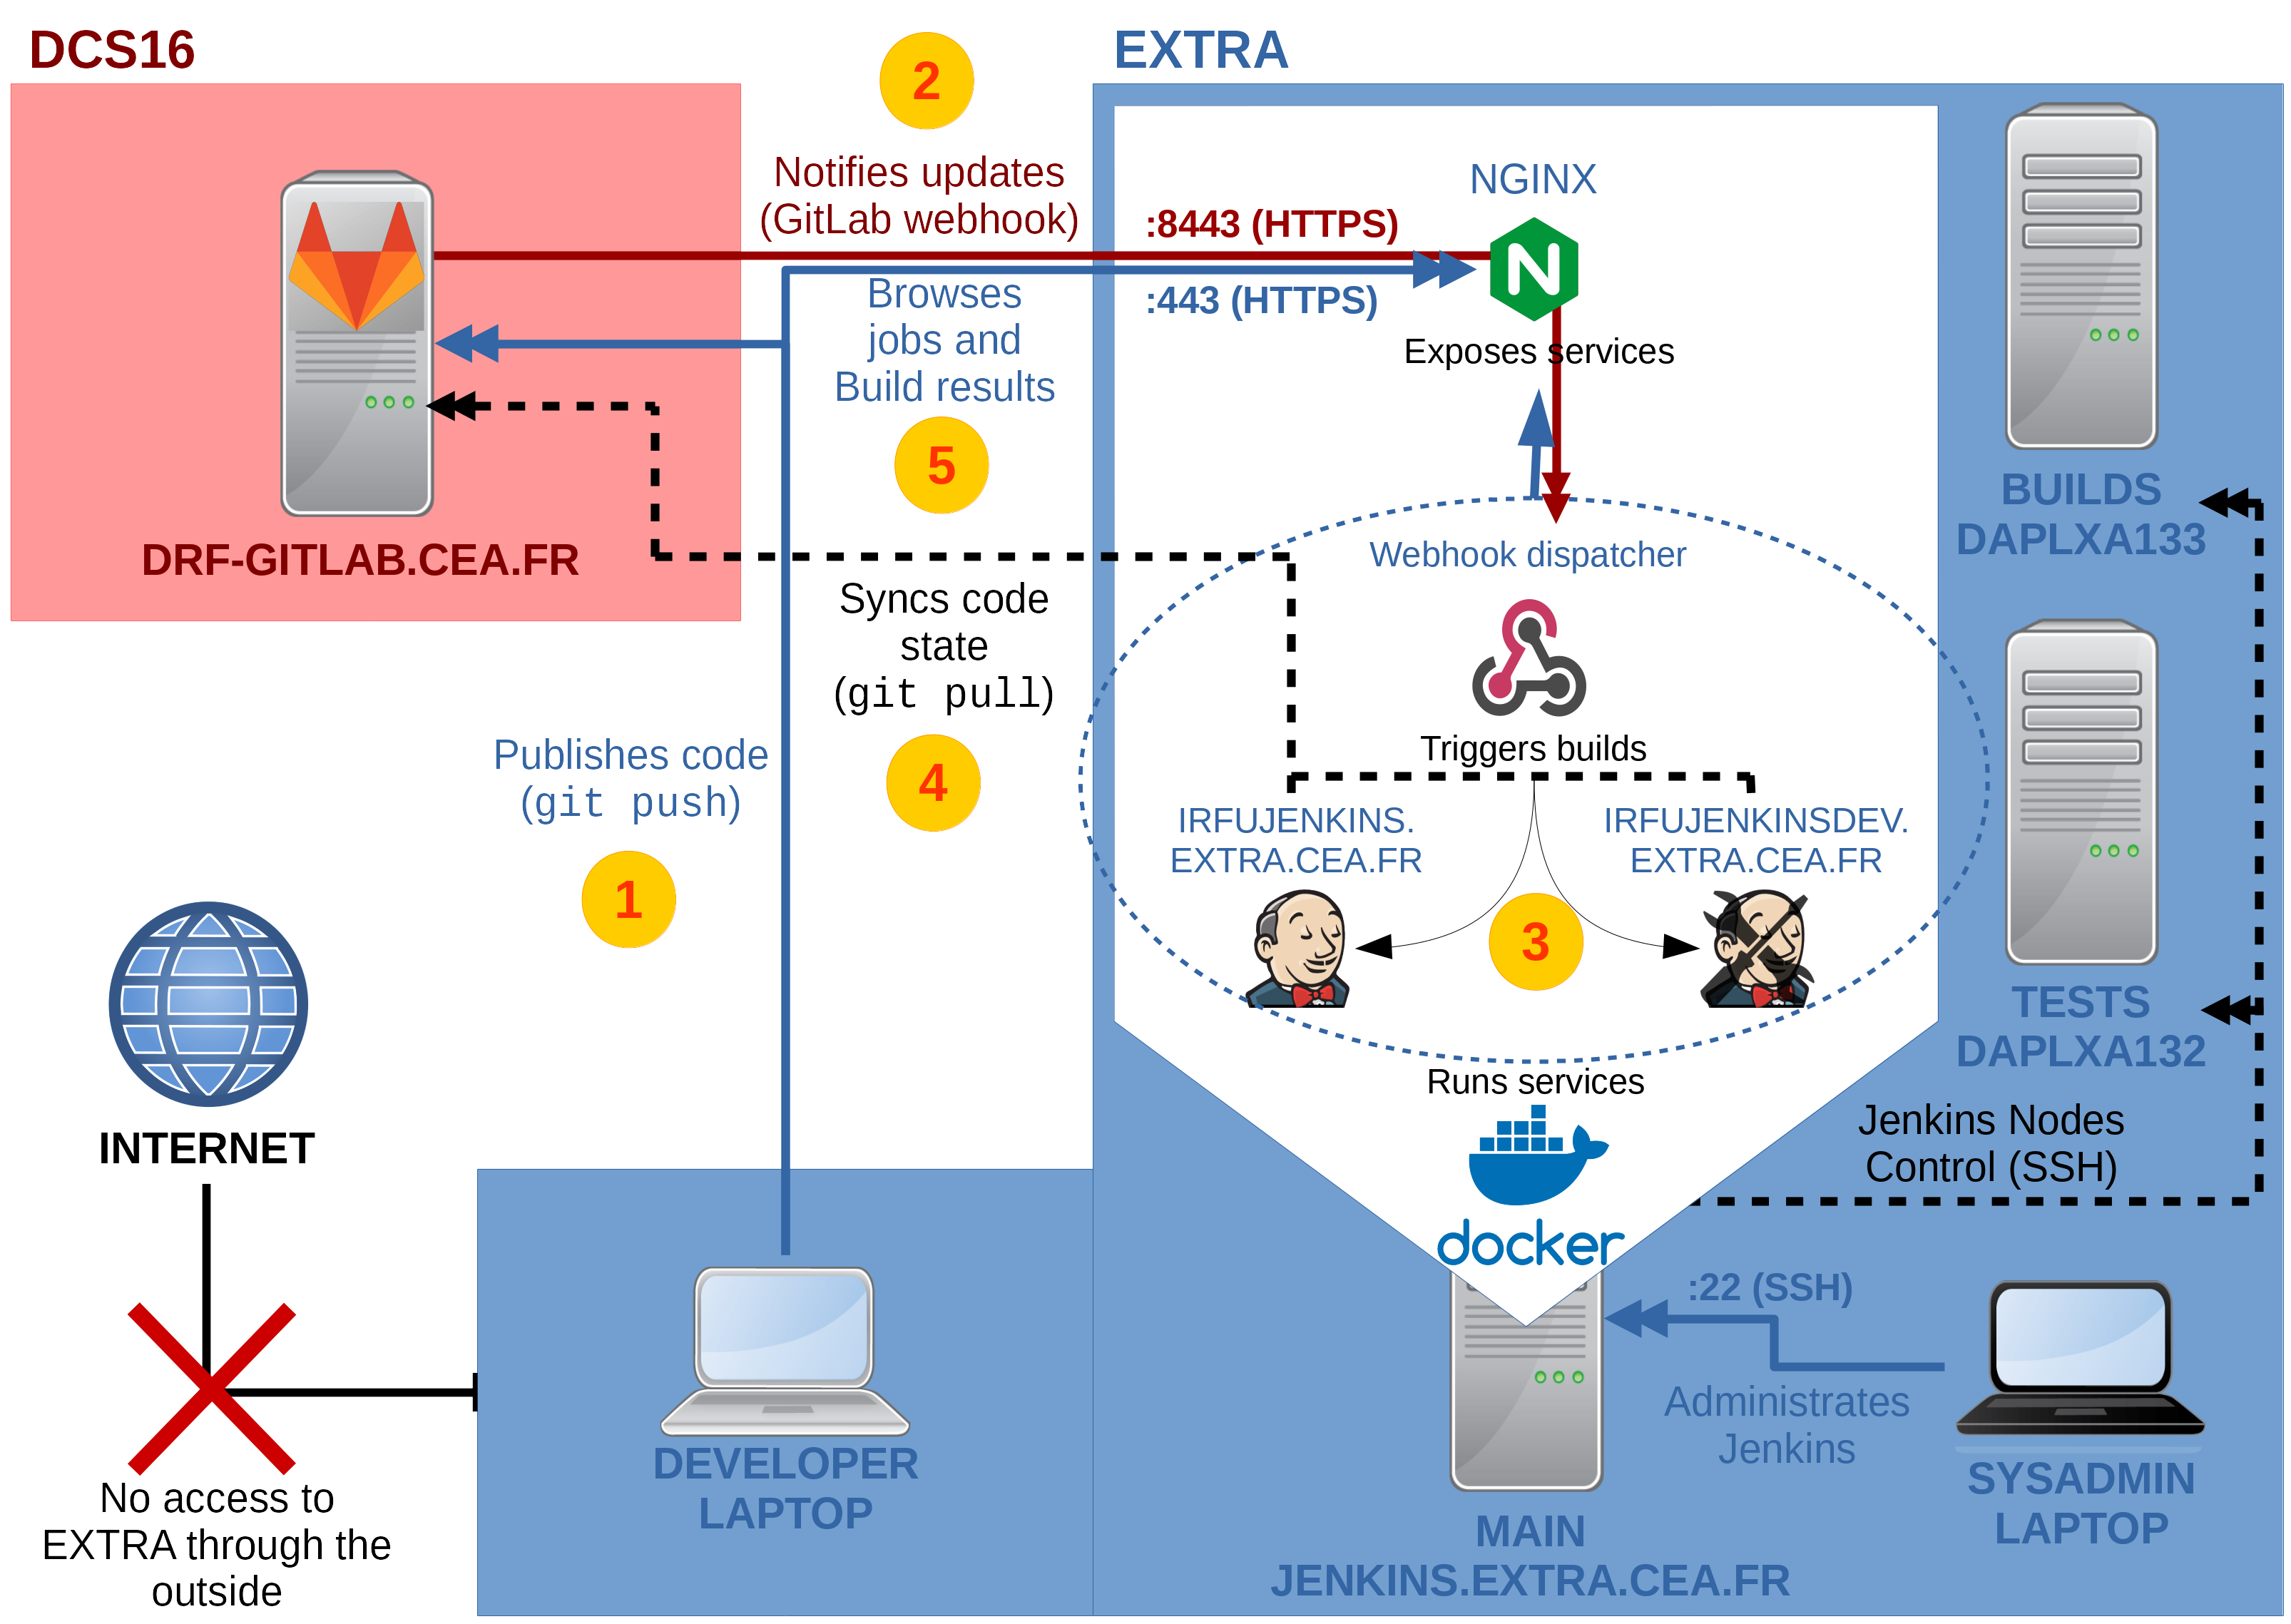
\includegraphics[width=\textwidth]{schema}\end{tikzfigure}
		  \begin{enumerate}
	\item Le développeur publie du code sur GitLab depuis sa machine de travail.
	\item GitLab notifie la plateforme d'une mise à jour.
	\item Jenkins déclenche un \textit{build} pour le \textit{job} concerné.
	\item Jenkins va récupérer la dernière version publiée du code source du projet, et exécute le \textit{pipeline}.
	\item Une fois l'exécution terminée, le développeur est notifié par e-mail. Il peut accéder à l'interface web de Jenkins pour avoir un retour sur le \textit{build}.
		  \end{enumerate}
  }

  %%%%%%%%%% ------------------------------------------ %%%%%%%%%%
  \blocknode%
  {Fonctionnalités automatisées}%
  {
		  \begin{itemize}
				  \item Compilation native sous Linux, compilation croisée pour la plateforme embarquée.
				  \item Tests unitaires, tests de couverture.
				  \item Analyse statique et contrôle des standards de codage.
				  \item Émission de rapports de métriques sous forme de graphiques.
				  \item Archivage des produits de la compilation.
		  \end{itemize}
  }

  %%%%%%%%%% ------------------------------------------ %%%%%%%%%%
  \blocknode%
  {Conclusion}%
  {
		  \begin{itemize}
				  \item Une approche concrète du génie informatique appliqué à un projet de recherche.
				  \item Réutilisation possible et probable de la plateforme pour le développement des logiciels de contrôle au sol du satellite.
				  \item Décollage prévu en 2021 depuis la Chine dans un lanceur Longue Marche 2C.
		  \end{itemize}
  }

\end{tikzpicture}

\end{document}
